\begin{frame}{Konfiguration für WiFi}
\begin{itemize}
 \item Kern konfigurieren
 \begin{itemize}
  \item firmware
 \end{itemize}
 \item WiFi aufsetzen
 \begin{itemize}
  \item Siehe {\bf 3-network} Wi-Fi 
 \end{itemize}
\end{itemize}
\end{frame}

\section{Kernel Konfiguration}

\begin{frame}{Konfiguration}{Network}
\begin{center}
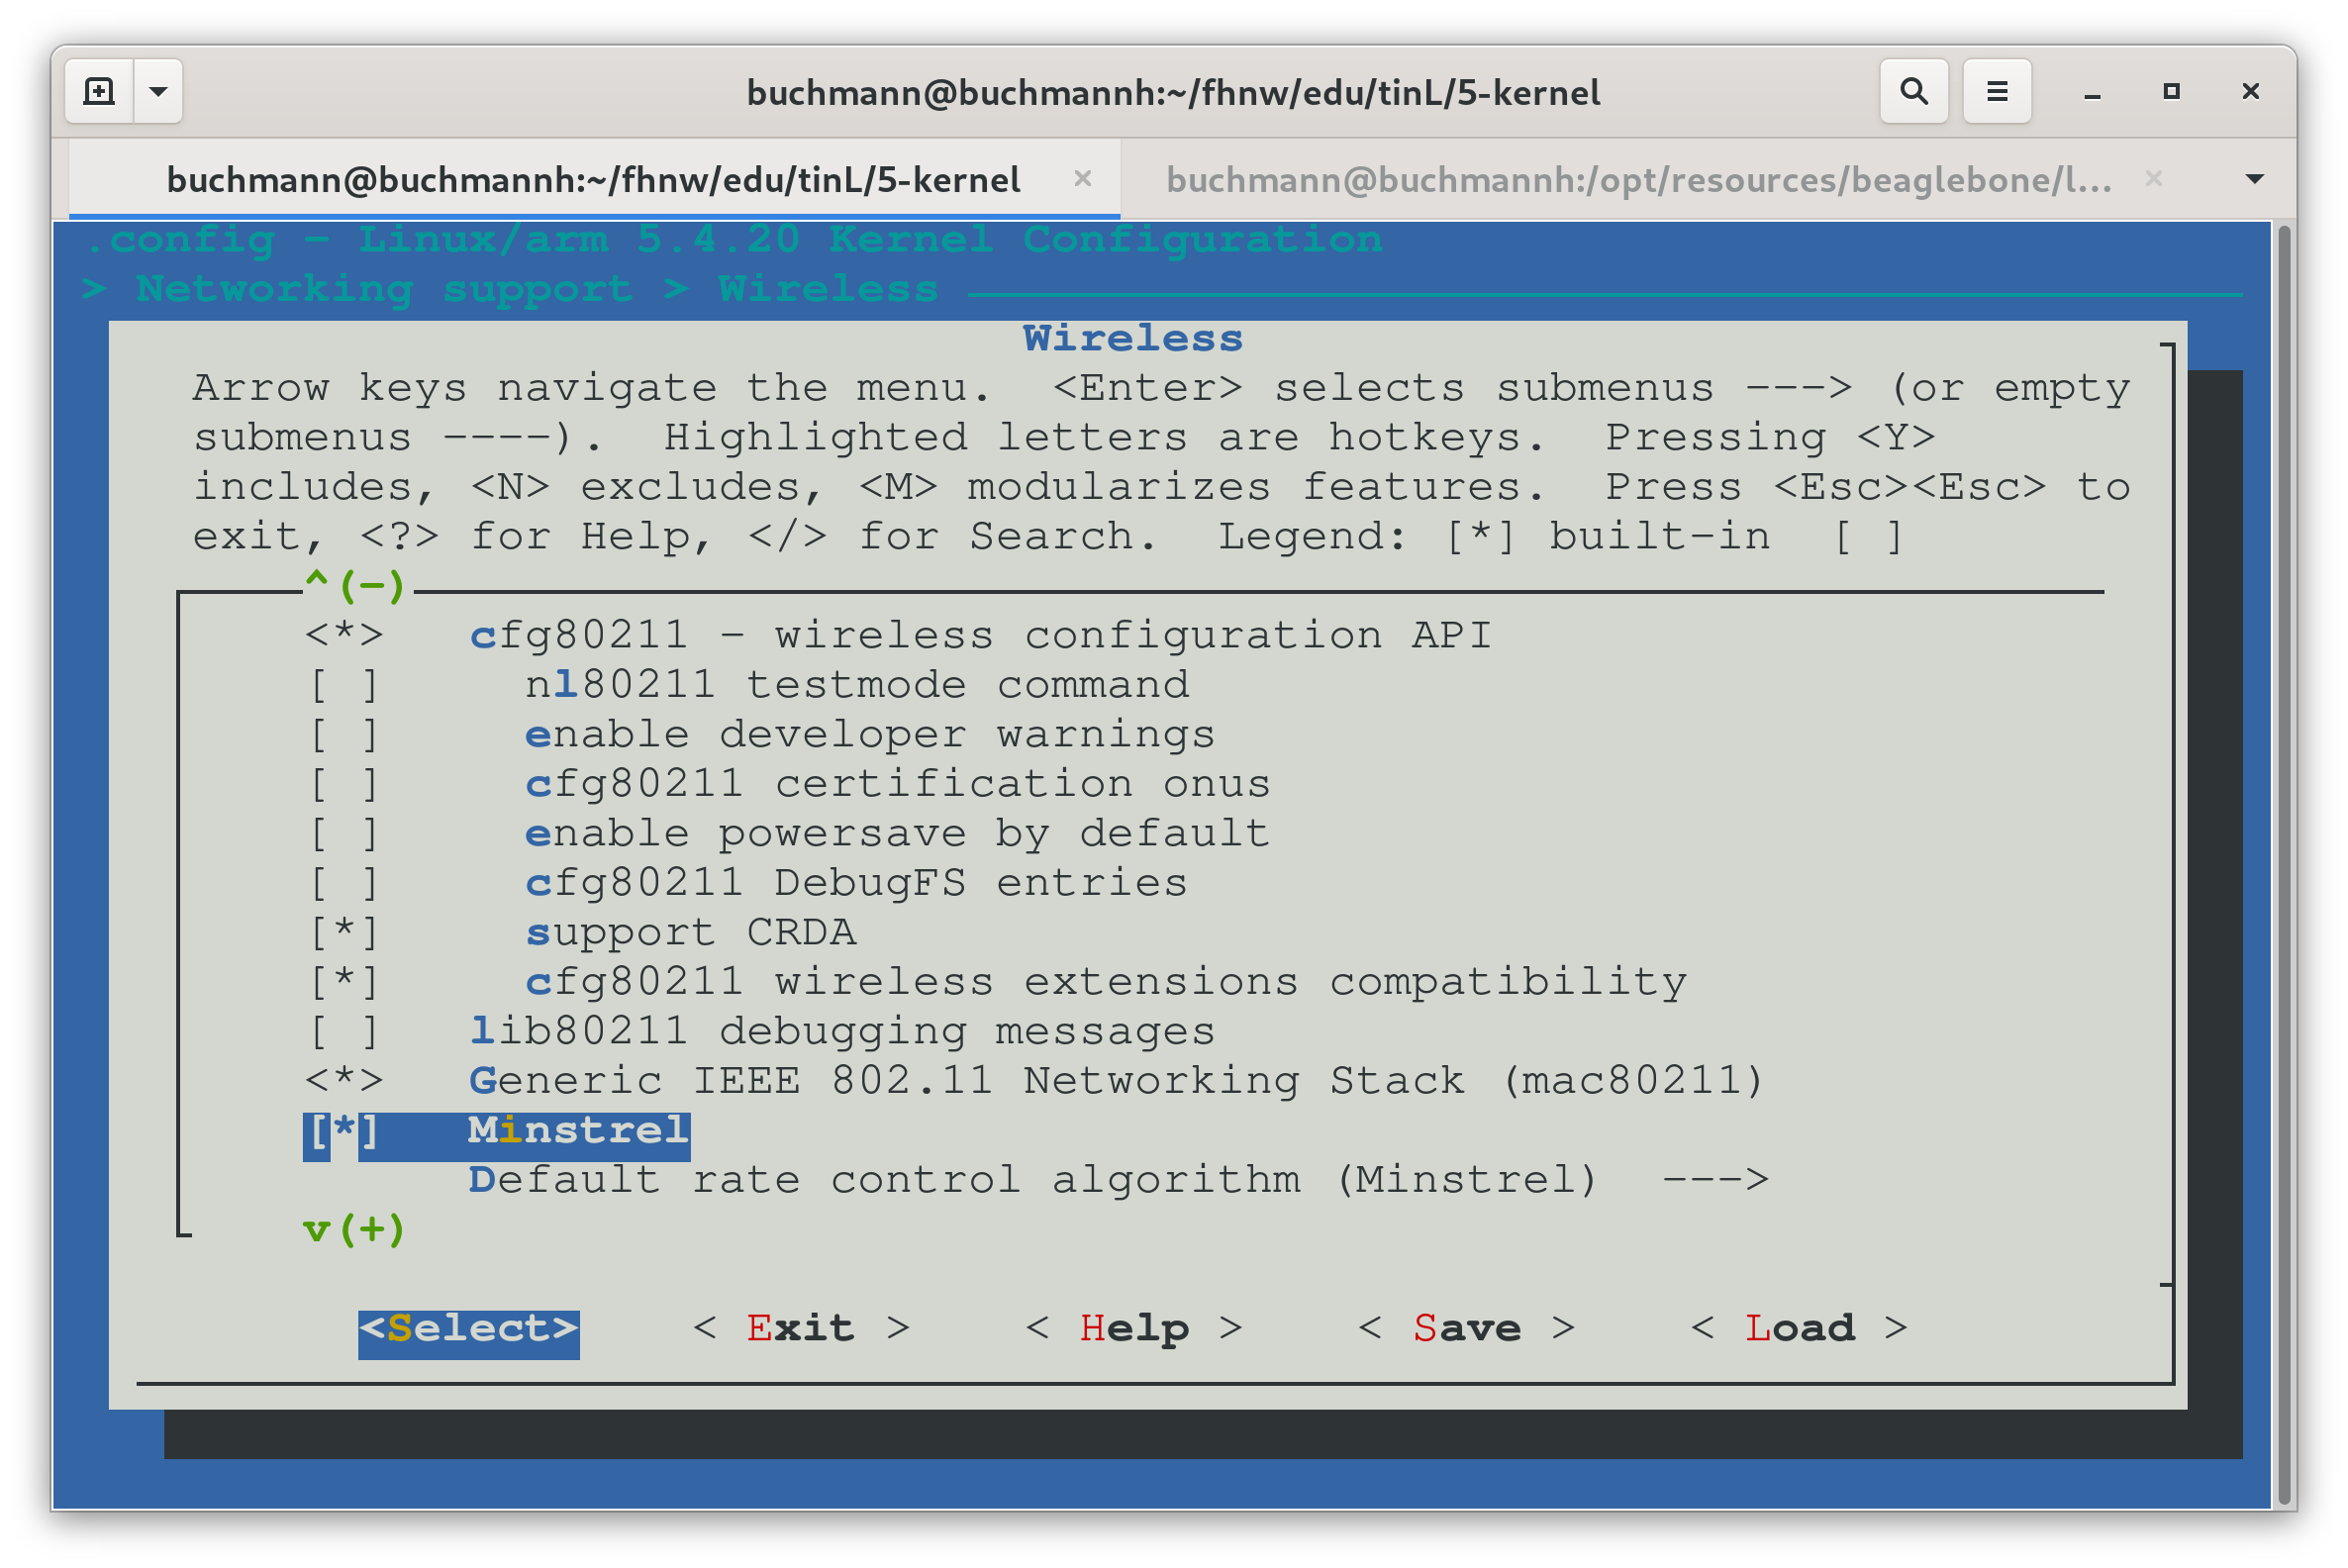
\includegraphics[width=0.75\textwidth]{wireless.png}
\end{center}
\end{frame}

\begin{frame}{Konfiguration}{Driver}
\begin{center}
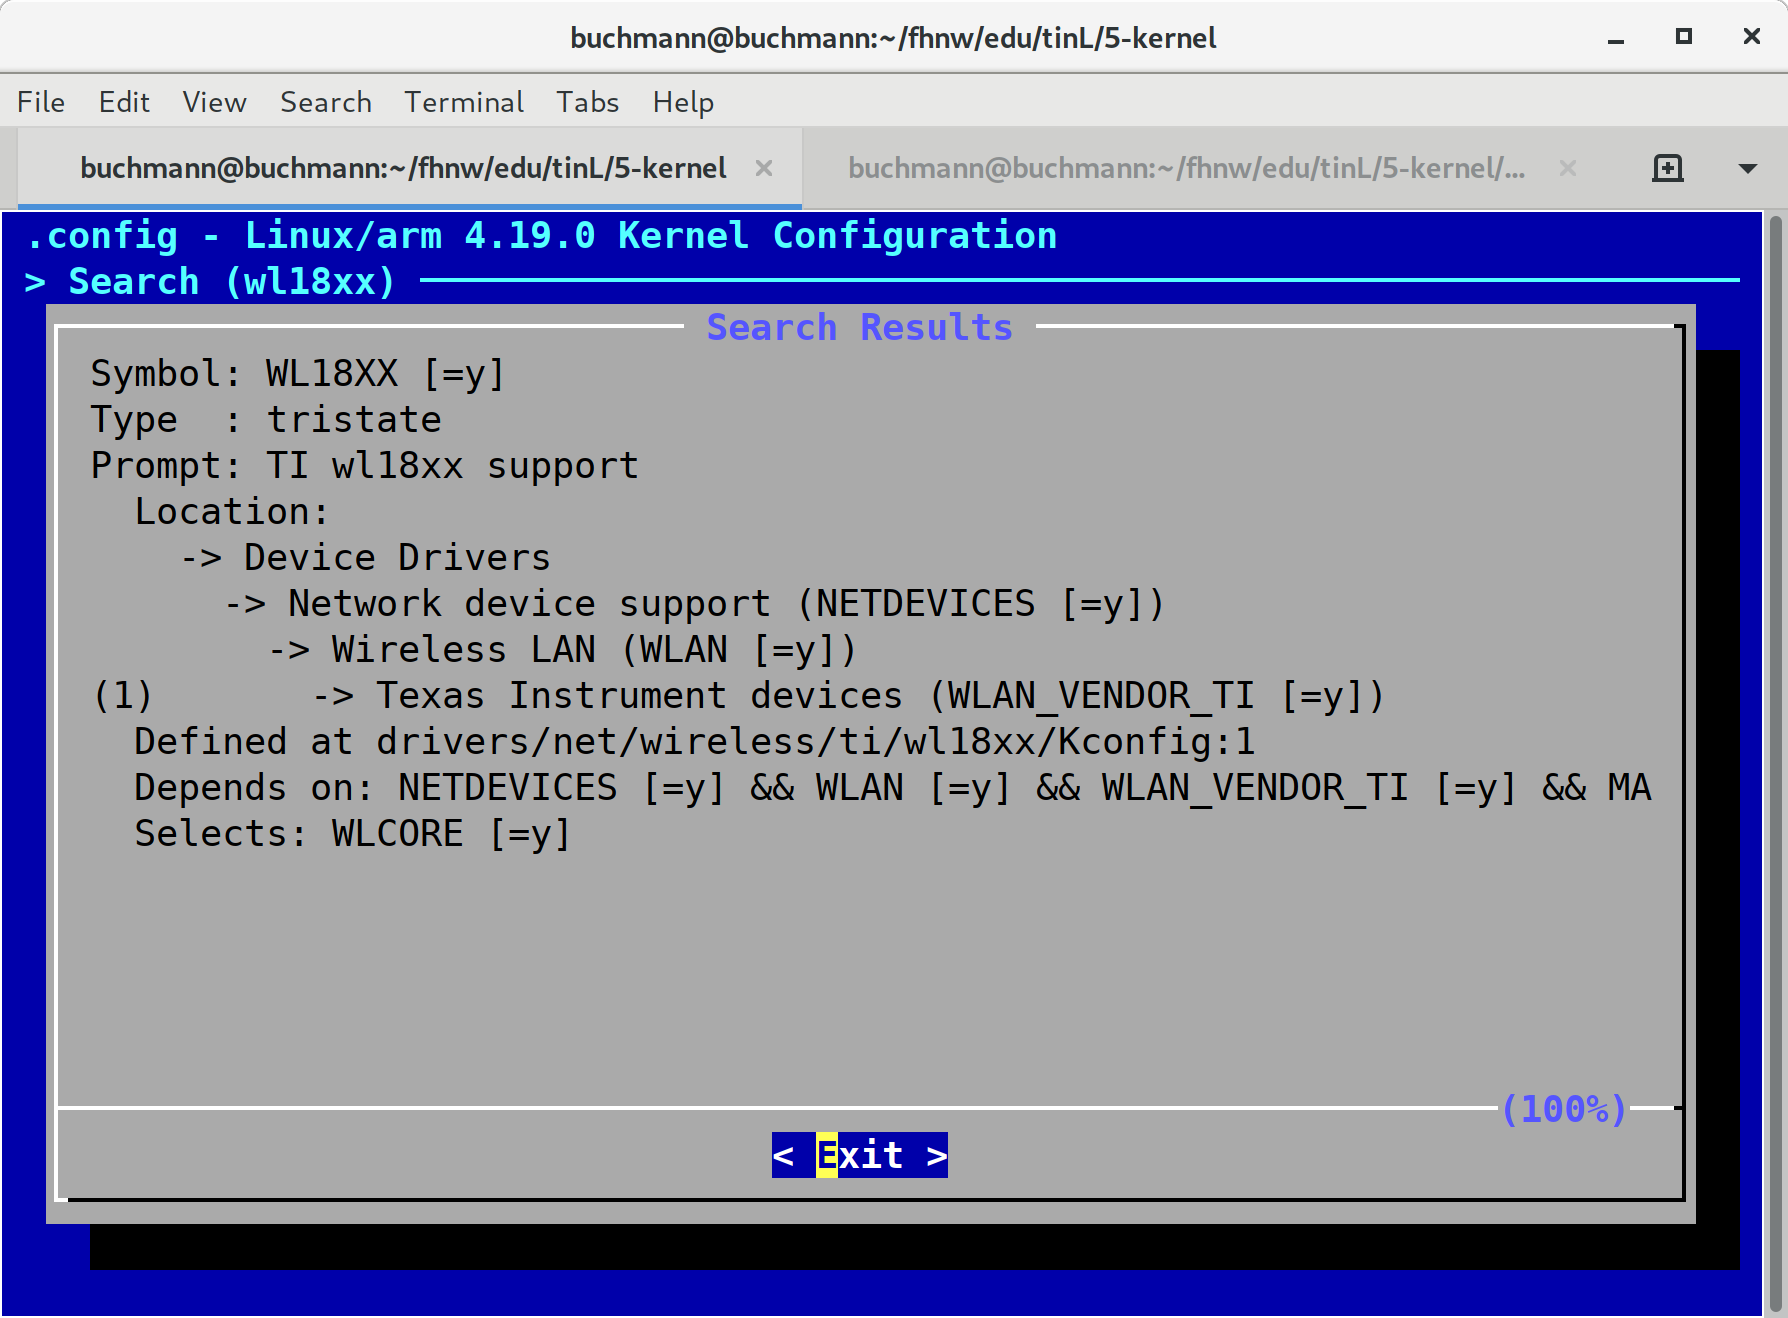
\includegraphics[width=0.75\textwidth]{wl18xx.png}
\end{center}
\end{frame}

\begin{frame}{Konfiguration}{Firmware}
\begin{center}
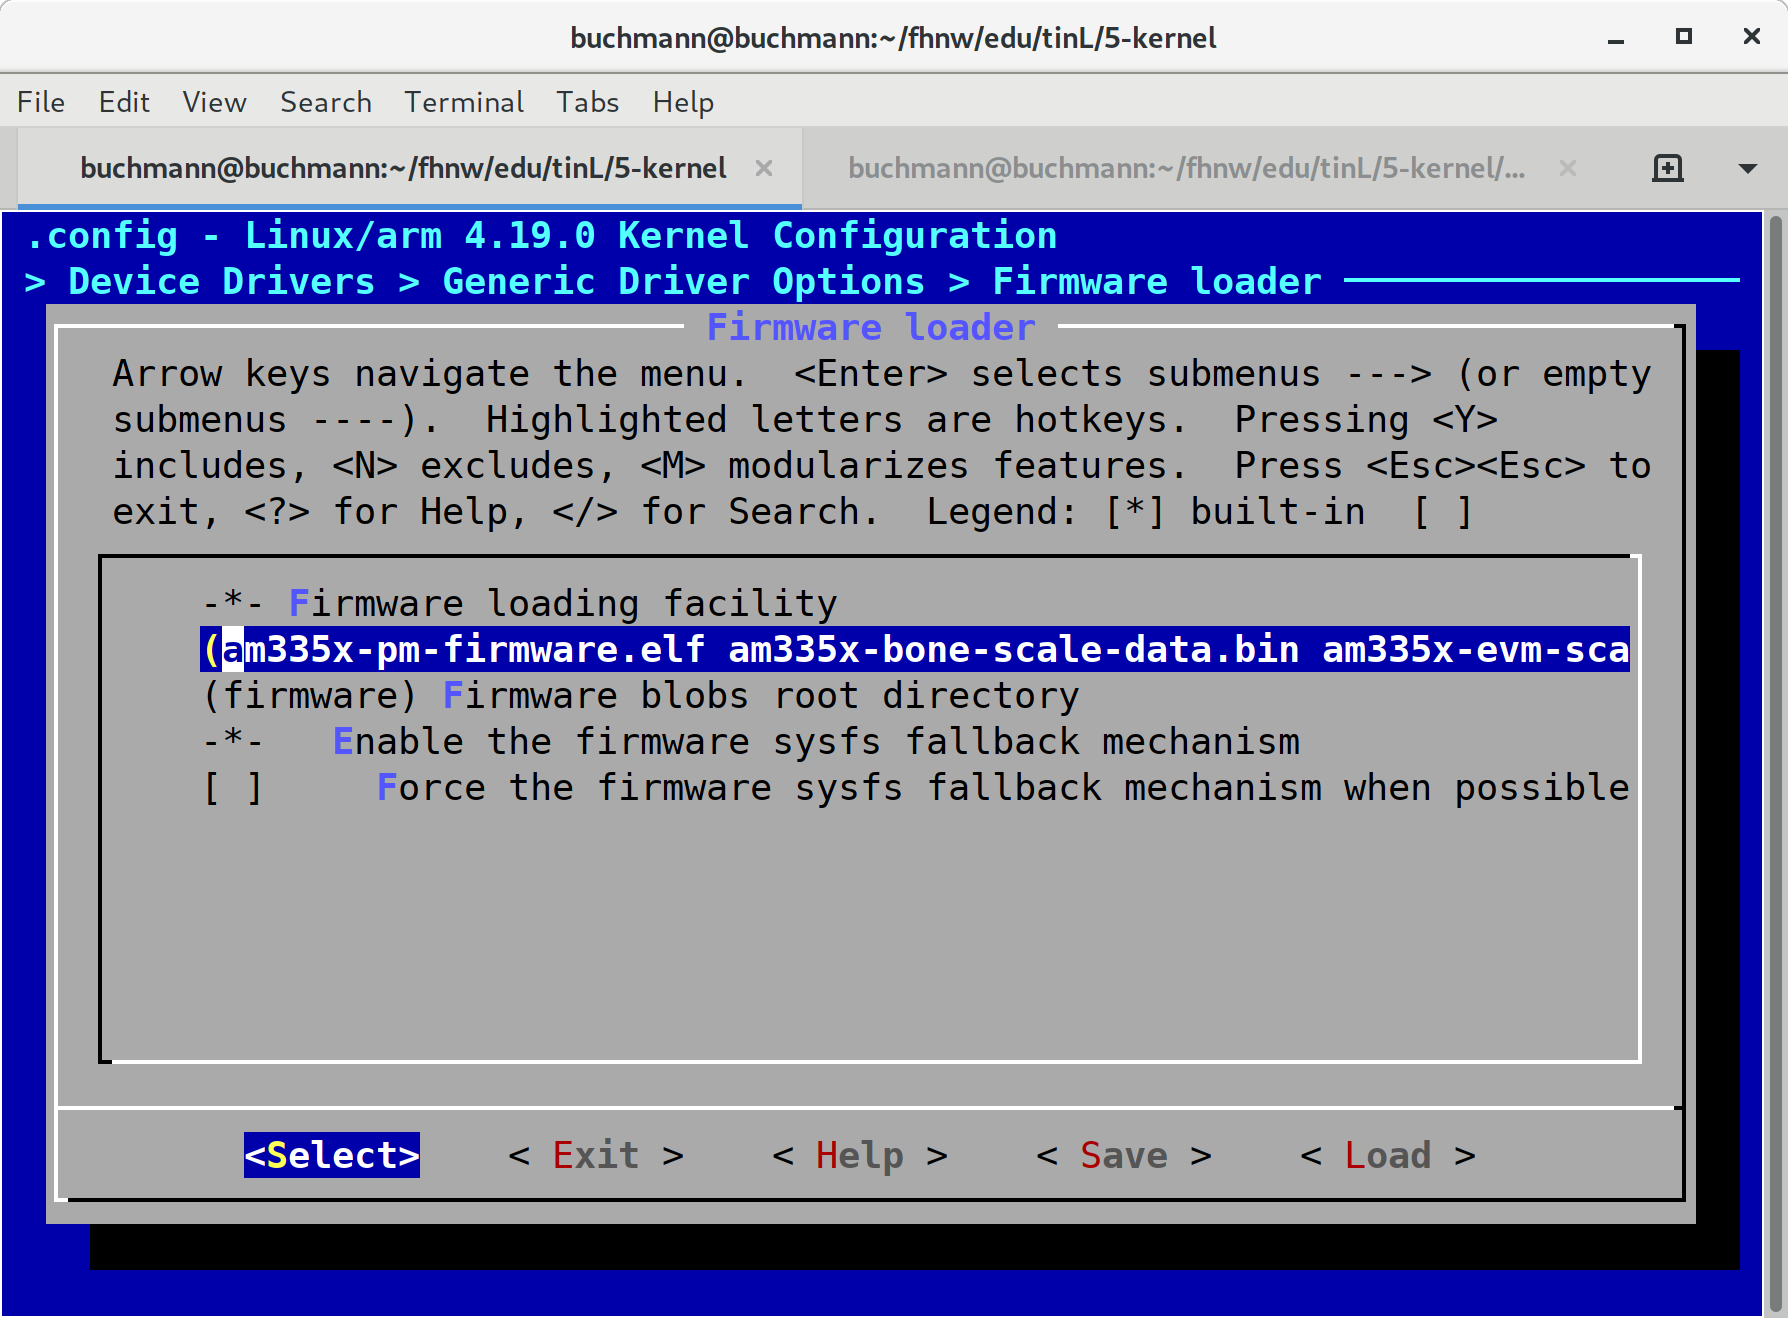
\includegraphics[width=0.75\textwidth]{firmware.png}
\end{center}
\end{frame}

\section{Wi-Fi aufsetzen}
\begin{frame}{Wi-Fi aufsetzen}
 \begin{itemize}
  \item \href{https://drive.switch.ch/index.php/s/b6kZ5n2TOIDzEiv}
        {target-root-2018.10.24.tar.gz}
        auf Partition 2 der SD Karte
  \item eigener {\em kernel} auf Partition 2 der SD Karte \cod{/boot}
  \item Siehe {\bf 3-network} 
 \end{itemize}
\end{frame}

\begin{frame}{Wi-Fi}
 \begin{block}{Basics}
  \begin{itemize}
   \item {\bf 3-network} Seite 14
  \end{itemize}
  \end{block}
  \begin{block}{Connect}
   \begin{itemize}
    \item {\bf 3-network} Seite 15
   \end{itemize}
 \end{block}
 \begin{block}{Internet}
  \begin{itemize}
   \item {\bf 3-network} Seite 16:\cod{udhcpc -i wlan0} 
   \item {\bf 3-network} Seite 12: route, DNS
  \end{itemize}
 \end{block}
\end{frame}

